% journal_ui_ana/english/src/20_pengembangan_hipotesis.tex
% This can be named 20_literature_review.tex or 20_related_work.tex if more appropriate
\section{Literature Review and Theoretical Background} % Title adjusted to be more general for a journal

Reverse engineering is a fundamental process in software analysis aimed at understanding the internal mechanisms of a system without access to its original source code \cite{Has18, gee24}. This process poses a significant threat to software security as it can be exploited to uncover proprietary algorithms, identify security vulnerabilities, pirate licenses, and even inject malicious code \cite{Wak24}. This vulnerability has driven the development of various protection techniques, including code obfuscation.

\subsection{Code Obfuscation Techniques}
Code obfuscation aims to transform program code into a functionally equivalent form that is significantly more difficult for humans to understand and analyze \cite{Jin24}. The goal is not to make reverse engineering impossible, but to increase the complexity and cost required, making it impractical for attackers. Obfuscation techniques can be classified based on the level of abstraction at which they are applied:

\subsubsection{Source Code Obfuscation}
Modifications are made to human-readable source code.
\begin{itemize}
    \item \bo{Layout Obfuscation:} Alters code appearance, such as scrambling variable and function names \cite{Cha04}, and removing whitespace and comments \cite{Bal11}. Provides minimal security against automated analysis.
    \item \bo{Data Obfuscation:} Hides data representation, for example, through string encoding \cite{Ert05, Fuk08, Kov13}, instruction substitution \cite{LeD12, Dar10}, or using mixed boolean-arithmetic expressions \cite{Liu21, Sch22, Zho07} to disguise data manipulation logic.
    \item \bo{Control Flow Obfuscation:} Modifies the program's execution path logic. Examples include inserting bogus control flow \cite{LiY211}, using opaque predicates \cite{XuD16}, and control flow flattening, which transforms structured code into a large and complex \code{switch} statement \cite{Lás09}.
\end{itemize}

\subsubsection{Bytecode Obfuscation}
This technique targets intermediate code such as Java bytecode, .NET CIL, or LLVM IR. Methods include identifier renaming, control flow obfuscation, string encryption, and inserting dummy code \cite{Pie18, Yak20}. Effective in complicating decompilation back to high-level source code.

\subsubsection{Binary Code Obfuscation}
Operates directly on machine-executable code.
\begin{itemize}
    \item \bo{Code Packing/Encryption:} Compresses or encrypts the original code, requiring a runtime stub to unpack/decrypt the code before execution \cite{Rou13}. Primarily hinders static analysis, but the original code is revealed in memory during execution.
    \item \bo{Control Flow Manipulation:} Uses indirect jumps/calls, modifies \code{call}/\code{ret} instructions, or breaks code into small blocks with jumps to disrupt linear disassembly and analysis \cite{Rou13}.
    \item \bo{Constant Obfuscation:} Hides constant values through arithmetic or logical operations \cite{Rou13}.
    \item \bo{Code Virtualization:} Considered one of the strongest binary obfuscation techniques, discussed further below.
\end{itemize}

\subsection{Code Virtualization (VM-Based Obfuscation)}
Code virtualization, or Virtual Machine (VM)-based obfuscation, is an advanced technique where segments of native machine code are translated into a custom bytecode format. This bytecode is then executed by a specially designed VM embedded directly into the application \cite{Ore06, Zho24}. As illustrated in Figure \ref{fig:jurnal_ui_ana_virtualization_process} from Oreans' research \cite{Ore06}, this process transforms the original code into a series of virtual instructions.

\begin{figure}[H]
	\centering
	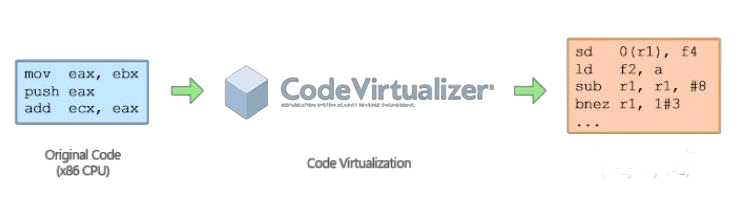
\includegraphics[width=0.7\textwidth]{\Assets/code_virtualization_process.png} % Assuming Assets is defined or path adjusted
	\caption{Code Virtualization Process \cite{Ore06}}
	\label{fig:jurnal_ui_ana_virtualization_process_en} % Unique label for the English journal
\end{figure}

The abstraction layer introduced by this VM creates a significant barrier for reverse engineers. Standard analysis tools cannot directly interpret the unique bytecode ISA \cite{Salwan2018SymbolicDeobfuscation}. Reverse engineers must first understand the VM's architecture, virtual instruction handler implementations, and bytecode mapping, a complex and time-consuming task \cite{Don20, Hac24}.

Key aspects of VM-based obfuscation include:
\begin{itemize}
    \item \bo{Custom ISA:} Each protected application can potentially have a unique or mutated set of virtual instructions, hindering signature-based detection or reuse of analysis results. Oreans \cite{Ore06} highlights the possibility of generating diverse VMs for different protected copies of an application.
    \item \bo{VM Architecture:} Typical VM components include fetch, decode, dispatch, and handler units, mimicking CPU operations but implemented in software \cite{Salwan2018SymbolicDeobfuscation, Hac24}. The complexity and implementation details of these handlers directly impact both security and performance. The execution flow of code virtualization can be seen in Figure \ref{fig:jurnal_ui_ana_execution_virtualization_en} (adapted from \cite{Don20}).

    \begin{figure}[H]
        \centering
        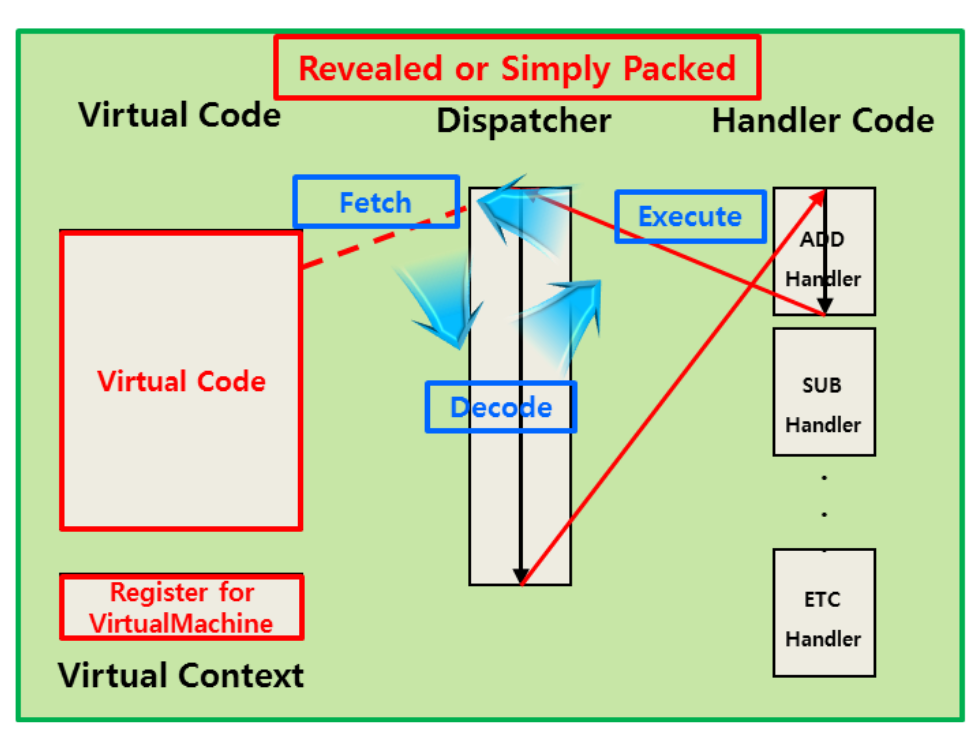
\includegraphics[width=0.6\textwidth]{\Assets/virtualization_execution.png}
        \caption{Code Virtualization Execution Flow (adapted from \cite{Don20})}
        \label{fig:jurnal_ui_ana_execution_virtualization_en}
    \end{figure}

    \item \bo{Security vs. Performance Trade-off:} The interpretation layer introduced by the VM inherently adds performance overhead compared to native execution. The level of obfuscation within the VM handlers and the complexity of the virtual instructions influence this trade-off.
\end{itemize}

Several commercial tools like VMProtect \cite{VMP24} and Themida \cite{Ore24} (which also includes virtualization features beyond basic packing) employ code virtualization. Academic research has also explored techniques such as symbolic deobfuscation to analyze virtualized code \cite{Salwan2018SymbolicDeobfuscation} and methods to enhance virtualization robustness, such as virtual code folding \cite{Don20}.

\subsection{Disassembly Techniques and Challenges}
Understanding the efficacy of binary obfuscation, particularly code virtualization, necessitates a brief overview of disassembly techniques. Disassemblers translate machine code into human-readable assembly language, forming a cornerstone of reverse engineering \cite{Sikorski2012}.

\subsubsection{Static Disassemblers}
Static disassemblers, such as Ghidra \cite{Nat19} and IDA Pro \cite{Hex91}, analyze executable files without running them. They employ techniques like linear sweep or recursive traversal to identify instruction sequences \cite{Eilam2011, Ko2007}. While comprehensive, static analysis struggles with code that is encrypted, packed, self-modifying, or significantly transformed, as the disassembler may misinterpret data as code or fail to follow the true control flow \cite{Sikorski2012, Blazytko2017}. Crucially, when faced with custom bytecode from a VM, static disassemblers designed for standard ISAs (e.g., x86-64) cannot correctly interpret these non-native instructions, leading to analysis failure.

\subsubsection{Dynamic Disassemblers}
Dynamic disassembly, typically a feature of debuggers like x64dbg \cite{Dun14}, occurs during program execution. The debugger disassembles instructions on-the-fly as they are about to be executed by the CPU. This approach can overcome some static analysis limitations, such as revealing unpacked or decrypted code in memory \cite{Sikorski2012}. Debuggers can also access runtime symbol information loaded by the operating system for system libraries, providing context for API calls. However, while a debugger can step through the native instructions of an embedded VM's interpreter, it will not directly reveal the original, pre-virtualized logic of the application. Instead, it shows the VM's internal operations executing the custom bytecode, which still obscures the application's core semantics from the analyst. These inherent limitations of standard disassembly tools underscore the challenge posed by advanced obfuscation techniques like code virtualization.

\subsection{VxLang in Context}
VxLang positions itself as a comprehensive framework offering binary protection, code obfuscation (including flattening), and code virtualization \cite{VxLang}. Its approach involves transforming native x86-64 code into an internal bytecode executed by its VM. This study aims to provide an empirical evaluation of the effectiveness of VxLang's virtualization component against standard reverse engineering practices and quantify its associated performance costs, thereby contributing practical insights into its utility as a software protection mechanism. Unlike analyzing established commercial protectors, this research focuses on the specific implementation and impact of the VxLang framework.
